% !TeX spellcheck = it_IT
\newpage
\section{Green Computing}
In generale, il green computing può aiutare le organizzazioni a ridurre l'impatto ambientale e a risparmiare sui costi energetici e di gestione.

\begin{definition}[Green Computing]
	Il green computing tratta la \textbf{progettazione}, la \textbf{realizzazione} e l'\textbf{utilizzo} di \underline{sistemi ICT}, \underline{computer} e \underline{dispositivi elettronici}\footnote{Tutti quei dispositivi che si appoggiano all'informatica per funzionare, e.g. aspirapolvere} in modo responsabile e sostenibile dal punto di vista ambientale, considerando in particolare il \textbf{consumo energetico} e \textbf{impronta di carbonio}.
\end{definition}

\begin{definition}[$CO_2$-eq]
	L'anidride carbonica equivalente è una misura che esprime l'impatto di una certa quantità di gas serra rispetto alla stessa quantità di anidride carbonica.
\end{definition}

\begin{definition}{Energy Star}
	Il progetto Energy Star nasce negli anni '90 ed è stata una delle prime iniziative relative al green computing per dare un indicatore dell'efficienza energetica. Il problema principale è che è \textbf{facoltativo}.
\end{definition}

\subsection{Approccio olistico}
Per funzionare segue un approccio \textbf{olistico}, analizzando tutto il \textbf{ciclo di vita} di un sistema, sia \emph{vericalmente} che \emph{orizzontalmente}.

\begin{itemize}
	\item \textbf{Progetto}: progettare in modo sostenibile computer, server, sistemi di raffreddamento e software a basso consumo e alta efficienza.
	\item \textbf{Produzione}: attenzione a non sprecare risorse limitate, ridurre gli scarti di fabbricazione e utilizzare fonti rinnovabili per la produzione.
	\item \textbf{Trasporto}: cercare di ridurre e ammortizzare l'uso di carburanti fossili sostituendoli con veicoli elettrici o ibridi e facendo spedizioni accorpate.
	\item \textbf{Uso}: utilizzare i sistemi cercando di ridurre il consumo con politiche di risparmio (e.g. ibernazione)
	\item \textbf{Dismissione}: lo smaltimento di dispositivi elettronici attraverso il riciclo
\end{itemize}

\subsection{Pilastri fondamentali}
\begin{center}
	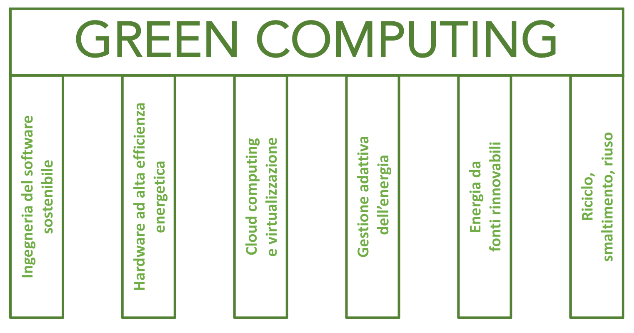
\includegraphics[scale=0.5]{green_pilastri.png}
\end{center}
\subsubsection{Ingegneria del software sostenibile}
È possibile fare in modo che i programmi consumino meno energia e che il loro dispiegamento nelle varie fasi del ciclo di vita produca minori gas inquinanti. In particolare, programmare \emph{sfruttando le peculiarità di linguaggi e hardware} che possano rendere il software più disponibile.
\subsubsection{Hardware ad alta efficienza energetica}
\subsubsection{Cloud computing e virtualizzazione}
\subsubsection{Gestione adattiva dell'energia}
\subsubsection{Energia da fonti rinnovabili}
\subsubsection{Riciclo, smaltimento, riuso}
È possibile \textbf{sensibilizzare} l'utente sul giusto uso dei mezzi a sua disposizione e quindi della loro conseguente fine di utilizzo. Ottimizzare l'impiego dei dispositivi porta una determinante longevità, minimizzando quindi il rifiuto.
\begin{itemize}
	\item Inoltre, per ridurre la produzione di rifiuti è fondamentale \textbf{riutilizzare} (ad esempio rivendendo) i dispositivi elettronici ancora validi. In molti casi è sufficiente sostituire componenti degradati (e.g. le batterie) e mantenere il resto. Oltretutto molti dispositivi possono essere considerati obsoleti per certi scopi ma ancora ottimi per altri (e.g. server).
	\item È fondamentale ingegnerizzare il processo di \textbf{smaltimento} in modo da permettere il \textbf{riciclo} di parte dei componenti. Ad esempio dalle schede stampate si possono recuperare metalli preziosi come l'oro. La legislazione italiana necessita il corretto trattamento dei rifiuti per ridurre l'inquinamento. Di conseguenza anche la scelta di macchinari e strumenti mirati allo smaltimento è fondamentale per fare in modo che un'azienda possa essere ritenuta green.
	\item La tecnologia stessa può essere uno strumento potente per \textbf{sensibilizzare} il consumatore su queste tematiche e per fargli conoscere le aziende green.
\end{itemize}
\subsection{Applicazioni green}
Sfruttare i sistemi ICT per l'\textbf{ottimizzazione} di processi che sfruttano risorse limitate (e.g. combustibili fossili nel trasporto, energia elettrica nel riscaldamento, acqua potabile nell'irrigazione) è un aspetto importante del green computing.

\section{Ebook reader}
Entro il 2025 si prevede che gli e-reader rappresenteranno circa il $75\%$ del mercato totale, anche se allo stesso tempo il numero di libri cartacei prodotti e  venduti è in continuo aumento.

\subsection{Ciclo di produzione}
Vediamo il ciclo di vita di un libro tradizionale cartaceo
\begin{center}
	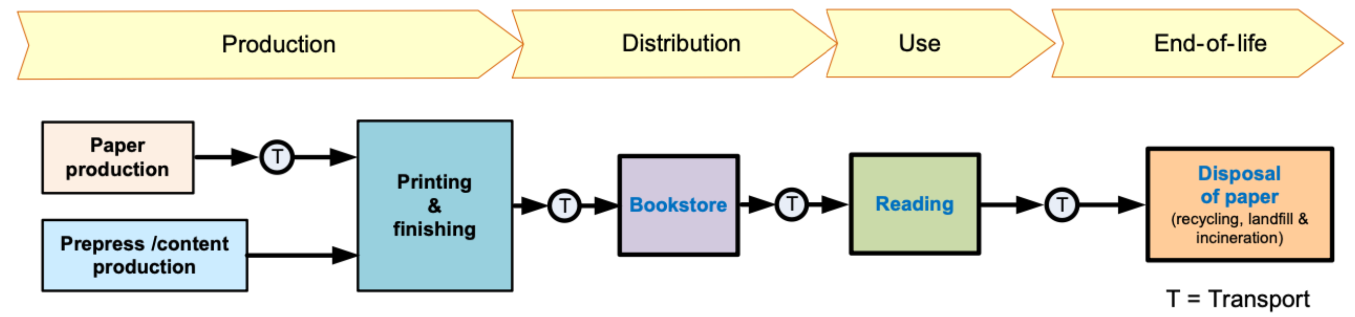
\includegraphics[scale=0.3]{books_lifecycle.png}
\end{center}
Le materie prime necessarie sono, per un libro a copertina morbida, $150-300$g di carta e $7.5$lt di acqua. Sono necessari $2$KWh  e la loro distribuzione (assumendo che non si usi la macchina per comprarlo) produce circa 10 volte quella della produzione. L'utilizzo è trascurabile dal punto di vista energetico in quanto al massimo serve una luce per leggere.
\begin{center}
	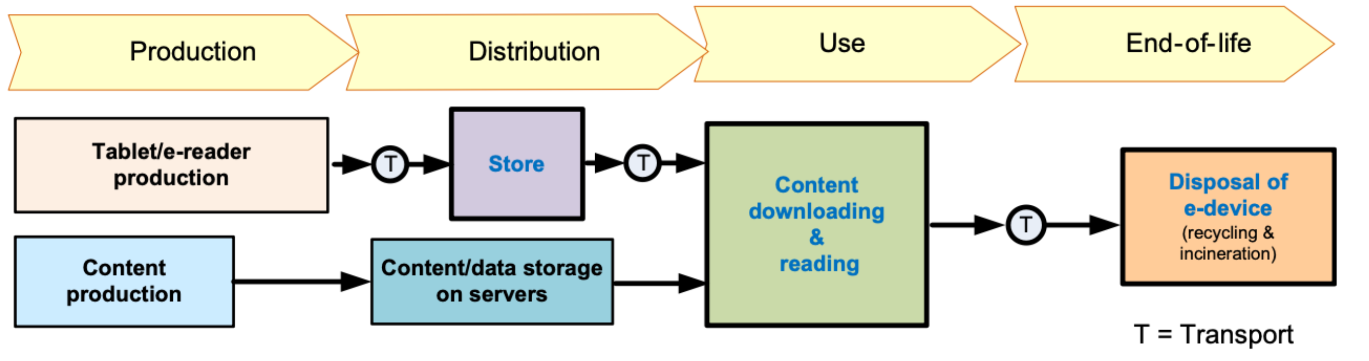
\includegraphics[scale=0.3]{ereader_lifecycle.png}
\end{center}
Per quanto riguarda invece gli e-book reader, sono necessari circa $15$Kg di materie prime (metalli rari, sabbia, etc...) e $300$lt di acqua (batterie, chip, oro dei circuiti). Sono necessari $100$KWh per la produzione e assumiamo i costi di distribuzione di un  \href{https://www.icao.int/environmental-protection/Carbonoffset/Pages/default.aspx}{\color{blue}volo Milano-Roma}.

\subsection{Confronto}
Considerando i dati precedenti:
\begin{enumerate}
	\item Quanti libri si producono con le materie prime necessarie per produrre un e-book reader?\\
	\begin{equation*}
		\frac{15Kg}{0.150Kg} = 100 \quad \frac{15Kg}{0.300Kg}=50
	\end{equation*}
	\item Quanti libri si producono con l'acqua necessaria per produrre un e-book reader?\\
	\begin{equation*}
		\frac{300lt}{7.5lt} = 40
	\end{equation*}
	\item Quanti libri si producono con l'energia necessaria per produrre un e-book reader?\\
	\begin{equation*}
		\frac{100KWh}{2KWh} = 50
	\end{equation*}
	\item Quanti libri serve produrre e trasportare per inquinare quanto per la produzione e il trasporto di un e-book reader?\\
	\begin{equation*}
		\begin{split}
			&\text{Produzione e-book reader}=0.319\frac{g}{Kw/h} \cdot 100Kw/h = 31.9Kg \quad \text{Distribuzione e-book reader}=41.8 Kg \\
			&\text{Totale e-book reader}=31.9Kg + 41.8Kg = 73.7 Kg \\
			&\text{Produzione libro}=0.319 \frac{g}{Kw/h} \cdot 2Kw/h = 0.638Kg \quad  \text{Distribuzione libro}= 0.638Kg \cdot 10 = 6.380Kg\\
			&\text{Totale libro}=6,380Kg + 0.638 Kg = 7.018Kg \\
			& \text{\textbf{Libri per e-book reader}}=\frac{73.7Kg}{7.018Kg}=10.5
		\end{split}
	\end{equation*}
	\item Qual'è la media dei valori delle risposte precedenti (quanti libri vale un e-book reader)?
	\begin{equation*}
		\frac{\frac{100+50}{2} + 40 + 50 + 10.5}{5} = 43.9
	\end{equation*}
	\item Quanti libri bisogna leggere all'anno per ammortizzare un e-book reader su 5 anni di vita media?
	\begin{equation*}
		\frac{43.9}{5} = 8.8
	\end{equation*}
\end{enumerate}

\subsection{Salute}
La produzione di libri ed e-book reader produce ossidi di azoto e zolfo %TODO FInisci

\subsection{Dismissione}
\begin{table}
	\begin{tabular}{|c|c|}
		\hline
		Libro & E-book reader \\
		\hline
		La \textbf{decomposizione} può generare il doppio delle emissioni e degli impatti tossici sulle falde acquifere rispetto alla sua intera produzione & In caso di smaltimento illegale in uno dei paesi in via di sviluppo, i lavoratori (spesso bambini) saranno esposti all'impatto tossico di alcune sostanza smantellate. \\
		Può essere prestato, regalato, donato ad una biblioteca oppure correttamente riciclato. & Se correttamente riciclato, molti materiali si potranno recuperare o smaltire correttamente.
	\end{tabular}
\end{table}
%TODO Formatta decentemente